%%%%%%%%%%%%%%%%%%%%%%%%%%%%%%%%%%%%%%%%%%%%%%%%%%%%%%%%%%%%%%%%%%%%%%%%%%%%
%%%%%%%%%%%%%%%%%%%%%%%%%%%%%%%%%%%%%%%%%%%%%%%%%%%%%%%%%%%%%%%%%%%%%%%%%%%%
\documentclass{beamer}
\usepackage[utf8]{inputenc}
\usepackage[spanish]{babel}
\usepackage{amsmath}
\usepackage{amsfonts}
\usepackage{amssymb}
\usepackage{graphicx}

\usepackage{bibentry}

\usepackage{movie15}

\usepackage{verbatim}
%\usepackage{authblk}

\usepackage{listings}
\usepackage{color}

%%%%%%%%%%%%%%%%%%%%%%%%%%%%%%%%%%%%%%%%%%%%%%%%%%%%%%%%%%%%%%%%%%%%%%%%%%%%
%%%%%%%%%%%%%%%%%%%%%%%%%%%%%%%%%%%%%%%%%%%%%%%%%%%%%%%%%%%%%%%%%%%%%%%%%%%%
\usetheme{Luebeck}
\usecolortheme{beaver}
{
%\usetheme{Luebeck}
%\setbeamercolor{palette secondary}{use=structure,fg=white,bg=red}
%\setbeamercolor{palette tertiary}{use=structure,fg=white,bg=green}
}

%
%
%
\definecolor{rojo}{rgb}{0.62353,0.10588,0.13725}
\definecolor{naranja}{rgb}{0.91765,0.23137,0.16078}
\definecolor{rosa}{rgb}{0.95294,0.53333,0.32157}
\definecolor{cafe}{rgb}{0.48627,0.14118,0.10196}
\definecolor{cafe2}{rgb}{0.243135,0.07059,0.05098}
\definecolor{cafe3}{rgb}{0.1215675,0.035295,0.02549}


\definecolor{UniBlue}{RGB}{83,121,170}
\setbeamercolor{title}{fg=white}
\setbeamercolor{frametitle}{fg=white,bg=rojo}
\setbeamercolor{structure}{fg=cafe,bg=rosa}

\setbeamercolor{alerted text}{fg=rosa,bg=cafe2}

\setbeamercolor{palette primary}{bg=rojo,fg=white}
\setbeamercolor{palette tertiary}{bg=cafe2,fg=white}
\setbeamercolor{palette quaternary}{use=structure,bg=cafe3,fg=white}
\setbeamercolor{itemize item}{bg=naranja,fg=white}
\setbeamercolor{section number projected }{bg=rosa,fg=white}

\setbeamertemplate{itemize item}{\color{naranja}$\bullet$}

%%%%%%%%%%%%%%%%%%%%%%%%%%%%%%%%%%%%%%%%%%%%%%%%%%%%%%%%%%%%%%%%%%%%%%%%%%%%
%%%%%%%%%%%%%%%%%%%%%%%%%%%%%%%%%%%%%%%%%%%%%%%%%%%%%%%%%%%%%%%%%%%%%%%%%%%%

%\DeclareUnicodeCharacter{00A0}{ }

\lstset{ %
%  language=R,                     % the language of the code
  basicstyle=\footnotesize,       % the size of the fonts that are used for the code
}


\theoremstyle{definition}
\newtheorem{defn}{Definici\'on}[section]

%%%%%%%%%%%%%%%%%%%%%%%%%%%%%%%%%%%%%%%%%%

\title[Pruebas de estacionariedad en series electrofisiol\'ogicas]
{Aplicaci\'on de pruebas de estacionariedad d\'ebil en series electrofisiol\'ogicas}

\author[Enciso Alva $\lvert$ Rodr\'iguez Torres $\lvert$ Tetlalmatzi Montiel]
{Erika Rodr\'iguez Torres, Margarita Tetlalmatzi Montiel \\ Julio Cesar Enciso Alva}

\institute[UAEH]
{Universidad Aut\'onoma del Estado de Hidalgo}

\date[Octubre 2016]
{49 Congreso Nacional de la SMM\\ 27 de Octubre de 2016}

\titlegraphic{
\hspace*{8cm}~

\includegraphics[width=9em]{./material1/SIGLAS_UAEH_02.png}
}

%%%%%%%%%%%%%%%%%%%%%%%%%%%%%%%%%%%%%%%%%%

%%%%%%%%%%%%%%%%%%%%%%%%%%%%%%%%%%%%%%%%%%%%%%%%%%%%%%%%%%%%%%%%%%%%%%%%%%%%
%%%%%%%%%%%%%%%%%%%%%%%%%%%%%%%%%%%%%%%%%%%%%%%%%%%%%%%%%%%%%%%%%%%%%%%%%%%%
\begin{document}

\frame{\titlepage}

\begin{frame}
\tableofcontents
\end{frame}

%\section{Introducci\'on}
%
%%%%%%%%%%%%%%%%%%%%%%%%%%%%%%%%%%%%%%%%%%%
%%%%%%%%%%%%%%%%%%%%%%%%%%%%%%%%%%%%%%%%%%%
%
%\begin{frame}\frametitle{Motivaci\'on}
%El estudio y diagnóstico de una gran cantidad de enfermedades depende de nuestra habilidad para
%registrar y analizar se\~nales electrofisiol\'ogicas. 
%
%\vspace{3em}
%
%Se suele asumir que estas se\~nales son complejas: no lineales, no estacionarias y sin equilibrio 
%por naturaleza. Pero usualmente no se comprueban formalmente estas propiedades.
%\end{frame}

%%%%%%%%%%%%%%%%%%%%%%%%%%%%%%%%%%%%%%%%%%%
%%%%%%%%%%%%%%%%%%%%%%%%%%%%%%%%%%%%%%%%%%%
%
%\begin{frame}\frametitle{El cuarteto de Anscombe}
%\begin{figure}[h]
%\centering
%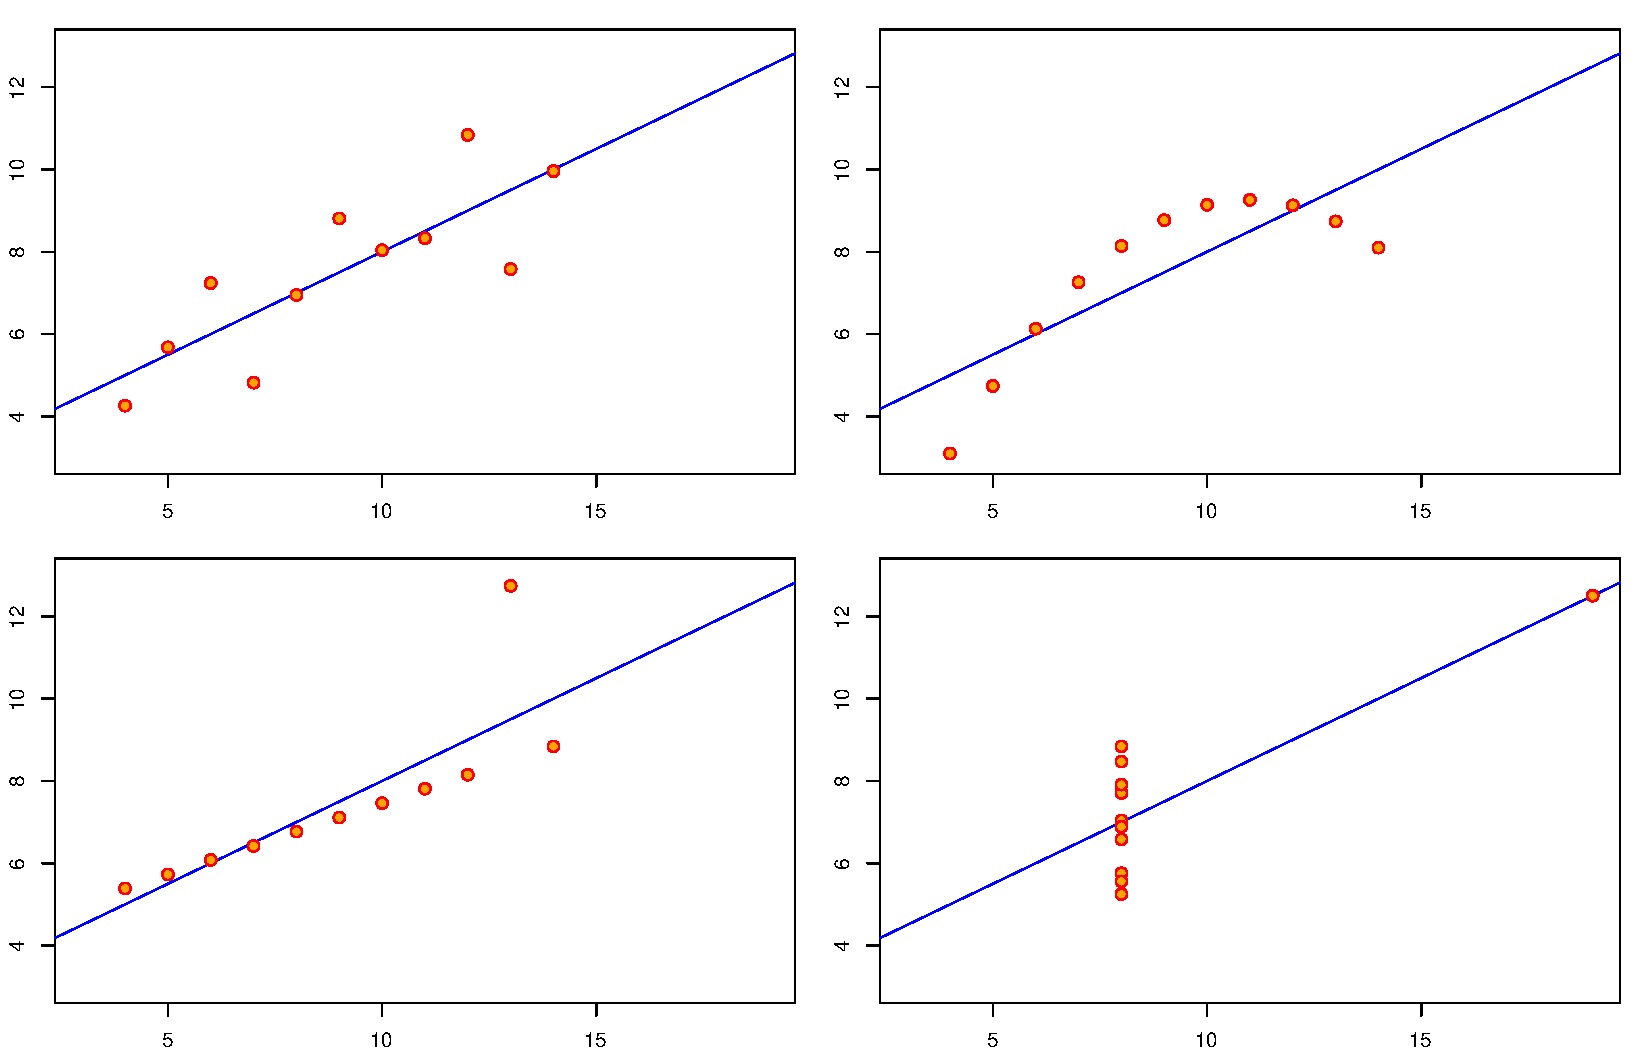
\includegraphics[width=0.8\linewidth]{./material1/anscombe.pdf} 
%\end{figure}
%\end{frame}
%
%%%%%%%%%%%%%%%%%%%%%%%%%%%%%%%%%%%%%%%%%%%
%%%%%%%%%%%%%%%%%%%%%%%%%%%%%%%%%%%%%%%%%%%

%\begin{frame}%\frametitle{Caracter\'istica buscada}
%\begin{defn}[Estacionariedad d\'ebil]
%Un proceso estoc\'astico $\{ X_t \}$, que satisface $E\left[ X_t^2 \right] < \infty$, 
%es \textbf{d\'ebilmente estacionario} si para todo tiempo $t$ se satisface que
%\begin{itemize}
%\item $E[X_t] = \mu < \infty$
%\item $Var\left[ X_t\right] =\sigma^2$
%\item Para todo $\tau\geq 1$, $Cov(X_t,X_{t+\tau}) = C(\tau)$
%\end{itemize}
%\end{defn}
%\end{frame}
%
%%%%%%%%%%%%%%%%%%%%%%%%%%%%%%%%%%%%%%%%%%%
%%%%%%%%%%%%%%%%%%%%%%%%%%%%%%%%%%%%%%%%%%%
%
%\begin{frame}\frametitle{Caso de estudio}
%Correlaci\'on inter-hemisf\'erica durante el sueño MOR del Adulto Mayor con Deterioro Cognitivo
%% sue\~no: atonia muscular, movimiento ocular r\'apido
%% parte frontal: toma de desiciones
%\begin{figure}[h]
%%\centering
%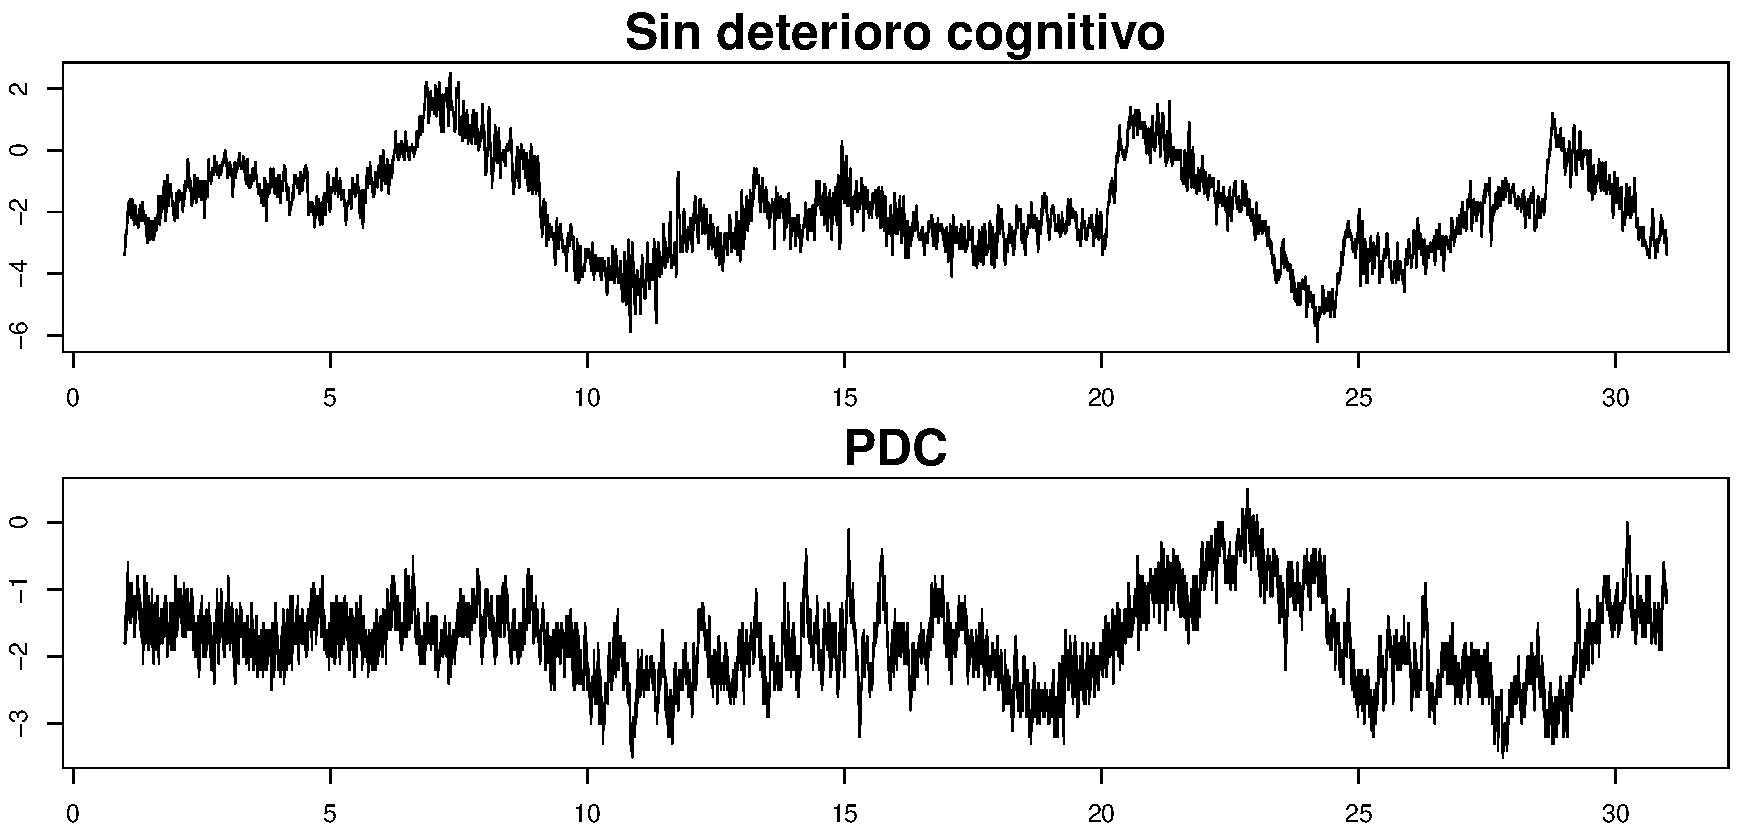
\includegraphics[width=0.5\linewidth]{./trabajo2/graficaintro.pdf}
%%\end{figure}
%%\begin{figure}[h]
%%\centering
%\includegraphics[width=0.5\linewidth]{./material1/cerebro.jpg}
%\end{figure}
%Adaptado de V\'azquez-Tagle y colaboradores (2016)
%\end{frame}
%
%%%%%%%%%%%%%%%%%%%%%%%%%%%%%%%%%%%%%%%%%%%
%%%%%%%%%%%%%%%%%%%%%%%%%%%%%%%%%%%%%%%%%%%
%
%\begin{frame}\frametitle{Registros de polisomnograma}
%\begin{figure}[h]
%\centering
%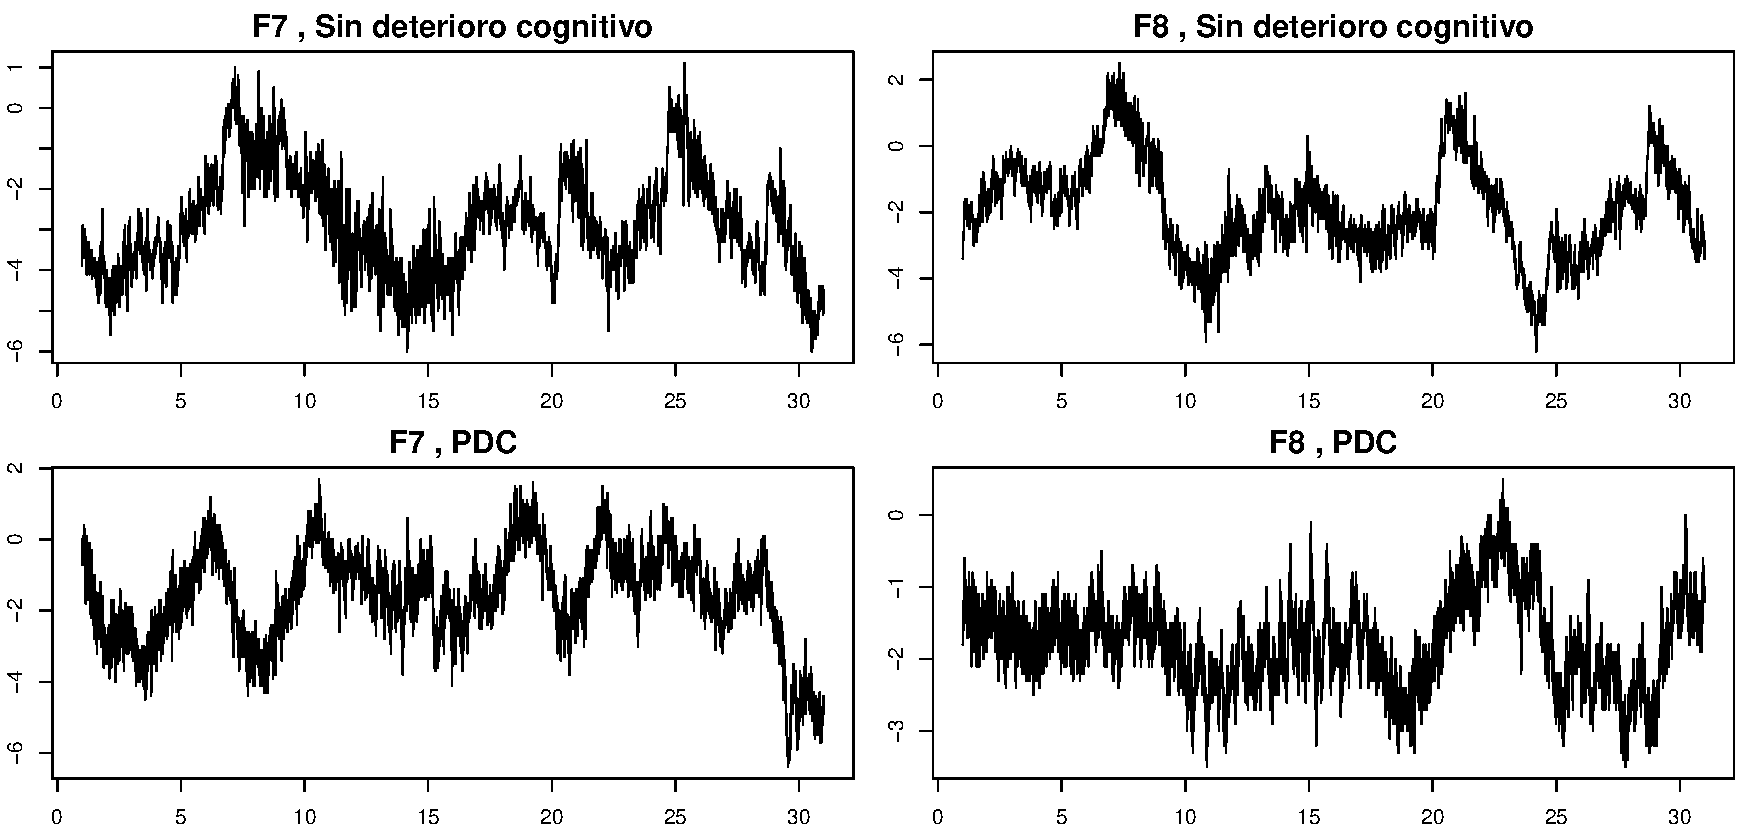
\includegraphics[width=\linewidth]{./trabajo2/estudio.pdf}
%\end{figure}
%\end{frame}
%
%%%%%%%%%%%%%%%%%%%%%%%%%%%%%%%%%%%%%%%%%%%
%%%%%%%%%%%%%%%%%%%%%%%%%%%%%%%%%%%%%%%%%%%
%
%\begin{frame}\frametitle{Prerrequisitos}
%Eliminar los efectos de:
%\begin{itemize}
%\item Tendencia
%\item Estacionalidad (\textit{seasonality})
%\end{itemize}
%\end{frame}
%
%%%%%%%%%%%%%%%%%%%%%%%%%%%%%%%%%%%%%%%%%%%
%%%%%%%%%%%%%%%%%%%%%%%%%%%%%%%%%%%%%%%%%%%
%
%\section[STL]{Seasonal Trend decomposition using Loess}
%
%\begin{frame}
%\frametitle{Descomposición cl\'asica usando loess}
%
%Filtro no-param\'etrico para generar las series de tiempo
%
%\begin{equation*}
%X_t = T_t + S_t + R_t
%\end{equation*}\\
%
%Tales que:\\
%\begin{description}
%\item[$S_t$] Función peri\'odica suave (frecuencia dada)
%\\ \textbf{Componente estacional}
%\item[$T_t$] Función suave, no necesariamente peri\'odica
%\\ \textbf{Tendencia}
%\item[$R_t$] Residuo
%\end{description}
%
%Comando en R: \textcolor{red}{\texttt{stl()}}
%\end{frame}
%
%%%%%%%%%%%%%%%%%%%%%%%%%%%%%%%%%%%%%%%%%%%
%%%%%%%%%%%%%%%%%%%%%%%%%%%%%%%%%%%%%%%%%%%
%
%\begin{frame}[fragile]
%\begin{figure}[h]
%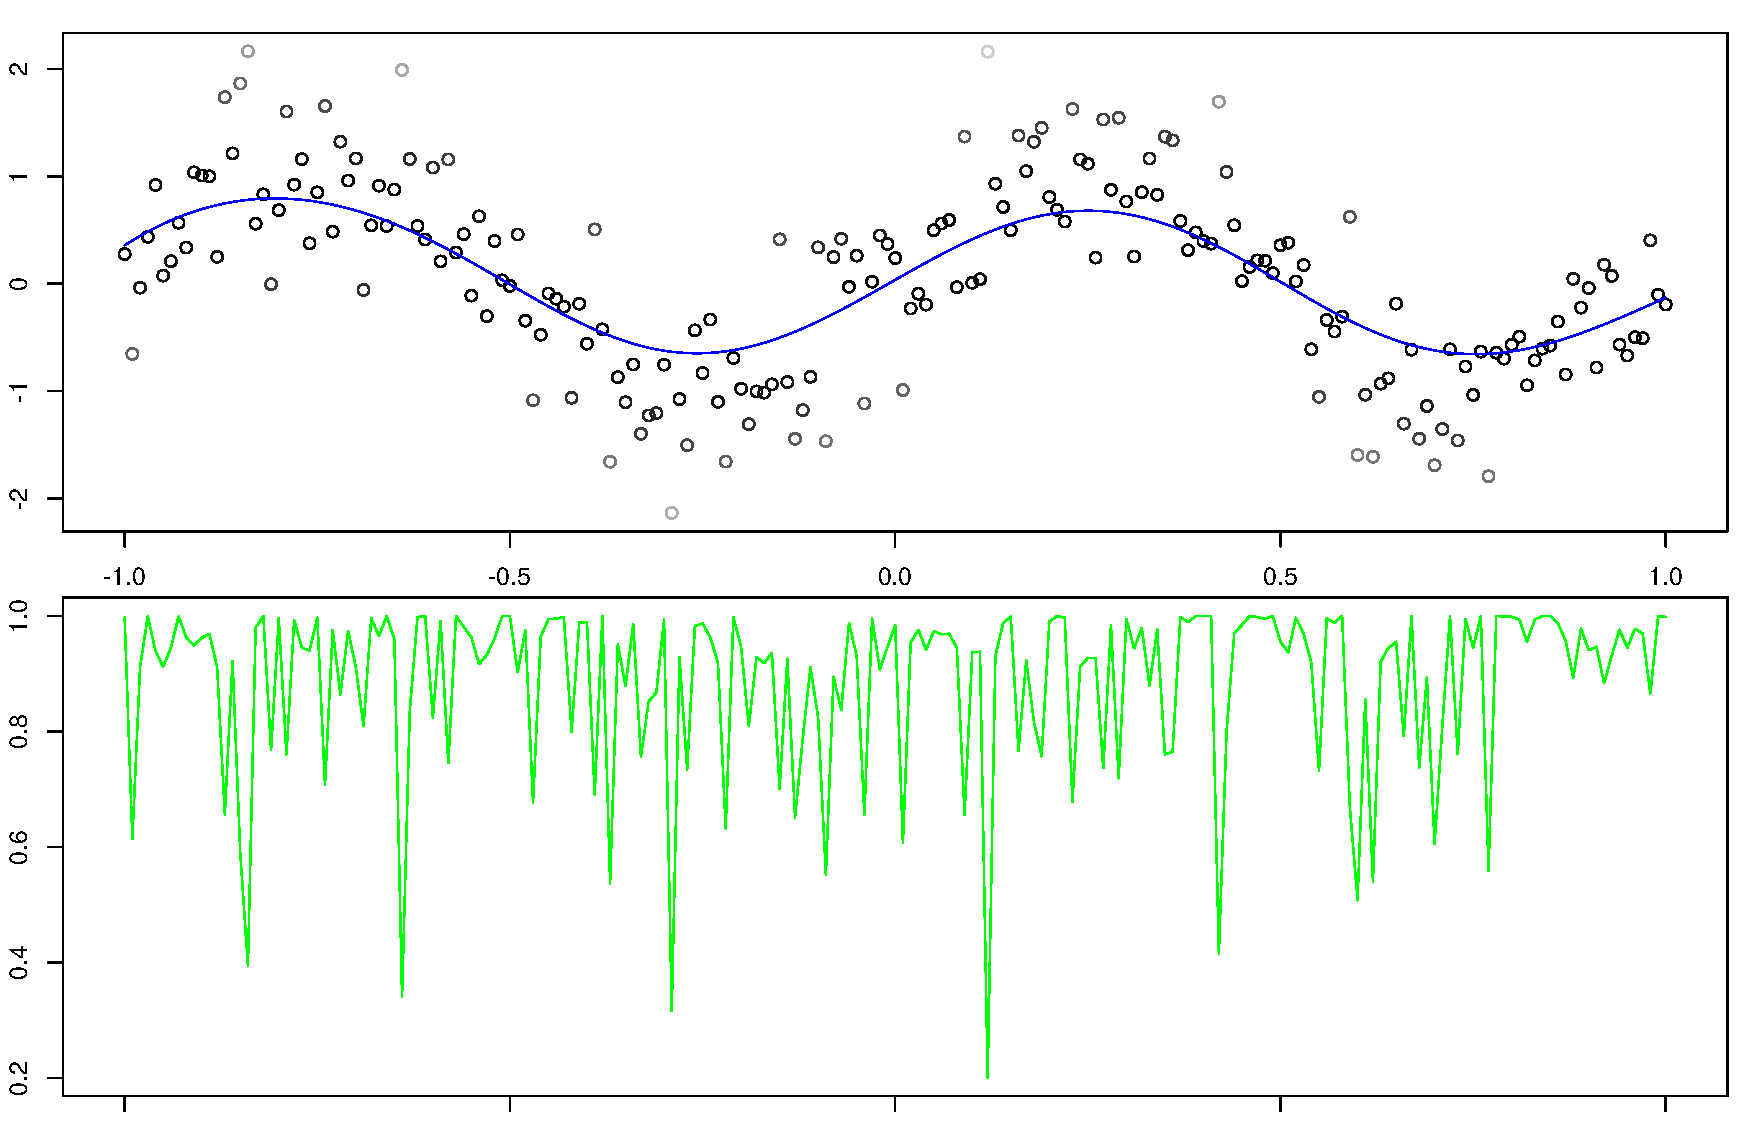
\includegraphics[width=\linewidth]{./trabajo2/stl_demo2_1.pdf} 
%\end{figure}
%\begin{center}
%\includemovie{3em}{3em}{./trabajo2/stl_demo2_gif.gif}
%\end{center}
%\end{frame}
%
%%%%%%%%%%%%%%%%%%%%%%%%%%%%%%%%%%%%%%%%%%%
%%%%%%%%%%%%%%%%%%%%%%%%%%%%%%%%%%%%%%%%%%%
%
%%\begin{frame}
%%\begin{figure}[h]
%%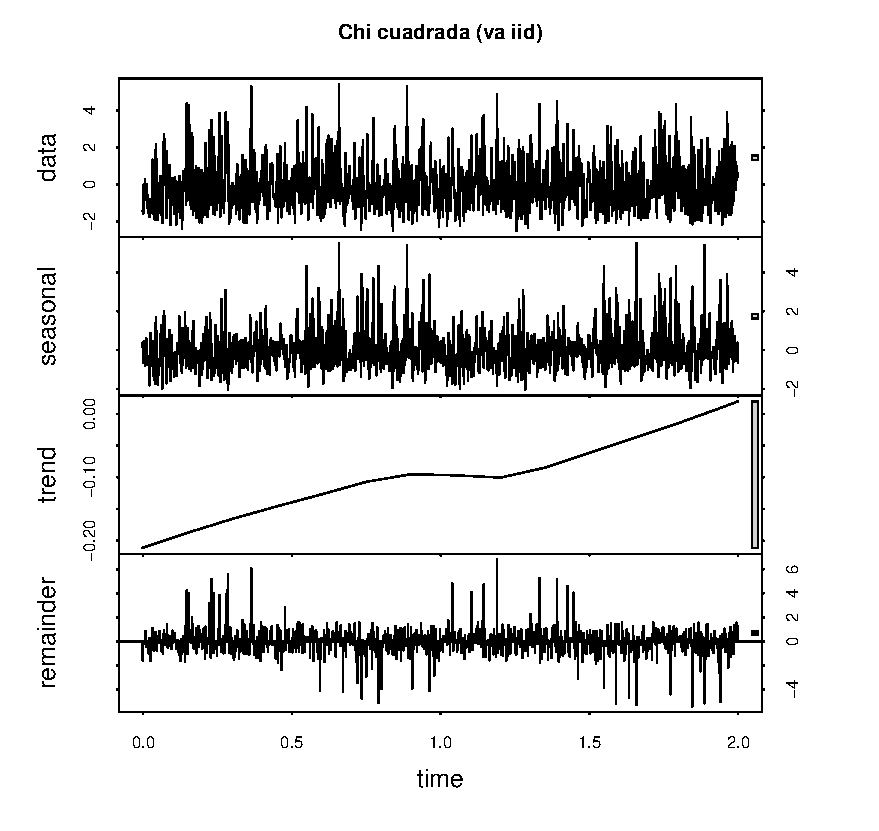
\includegraphics[width=0.5\linewidth]{./trabajo2/stl_1.pdf} 
%%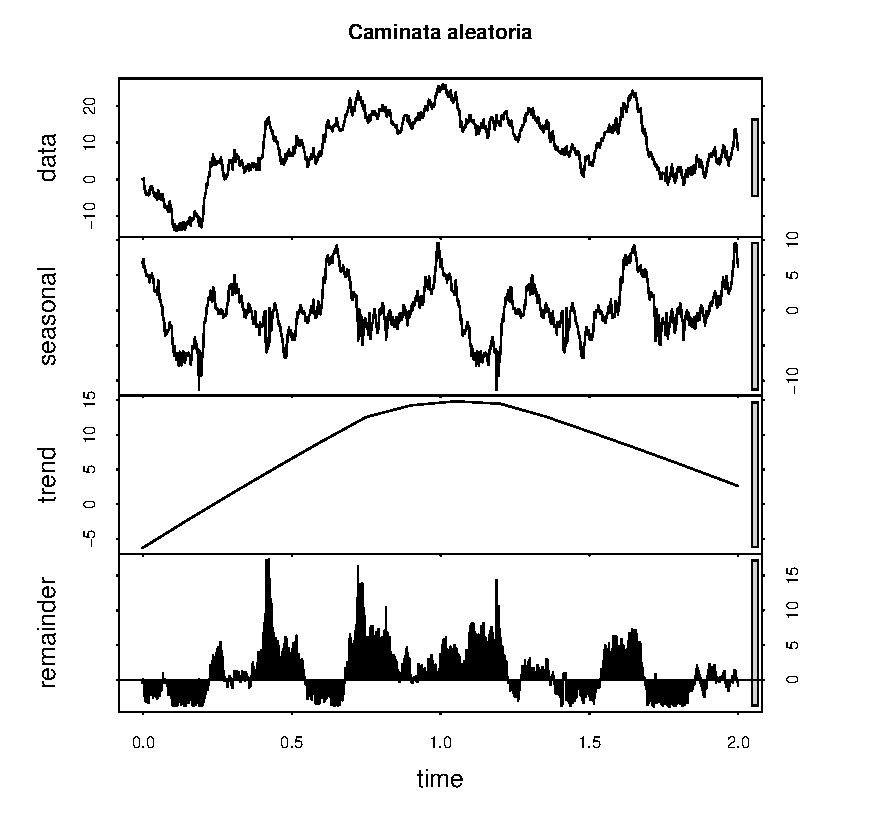
\includegraphics[width=0.5\linewidth]{./trabajo2/stl_2.pdf} 
%%\end{figure}
%%\end{frame}
%
%
%\begin{frame}\frametitle{Casos de estudio: sin deterioro}
%\begin{figure}[h]
%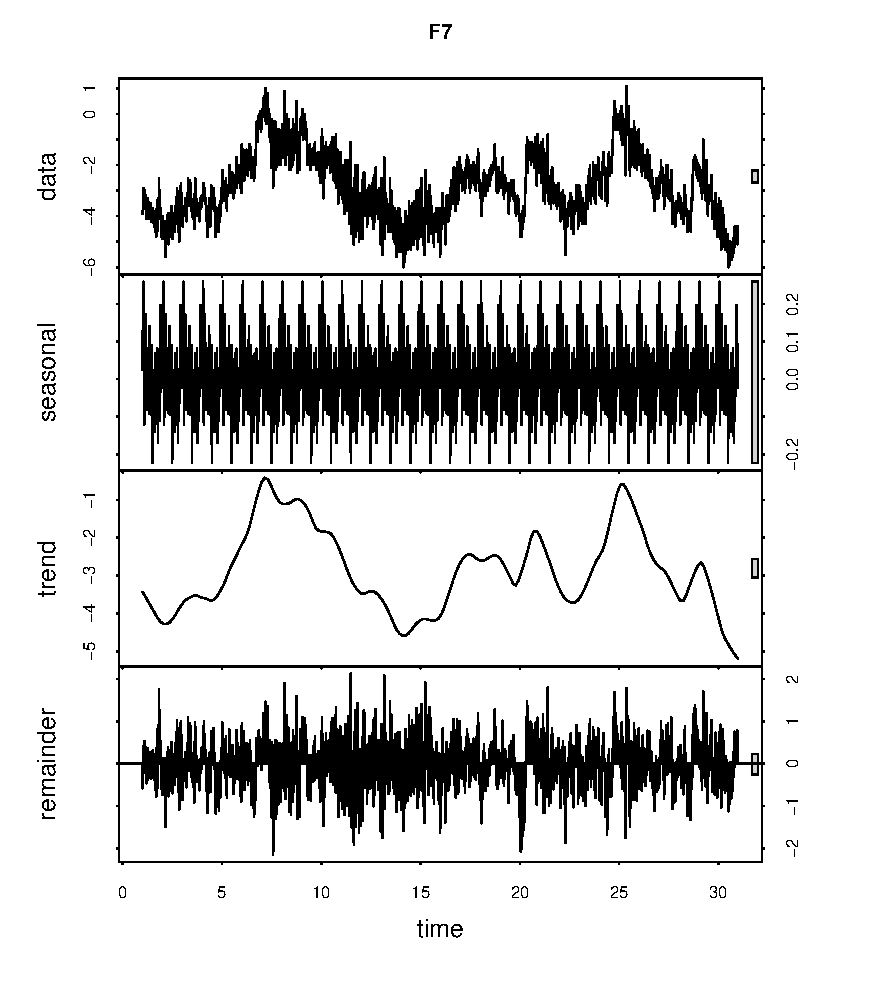
\includegraphics[width=0.5\linewidth]{./trabajo2/stl_n_f7.pdf} 
%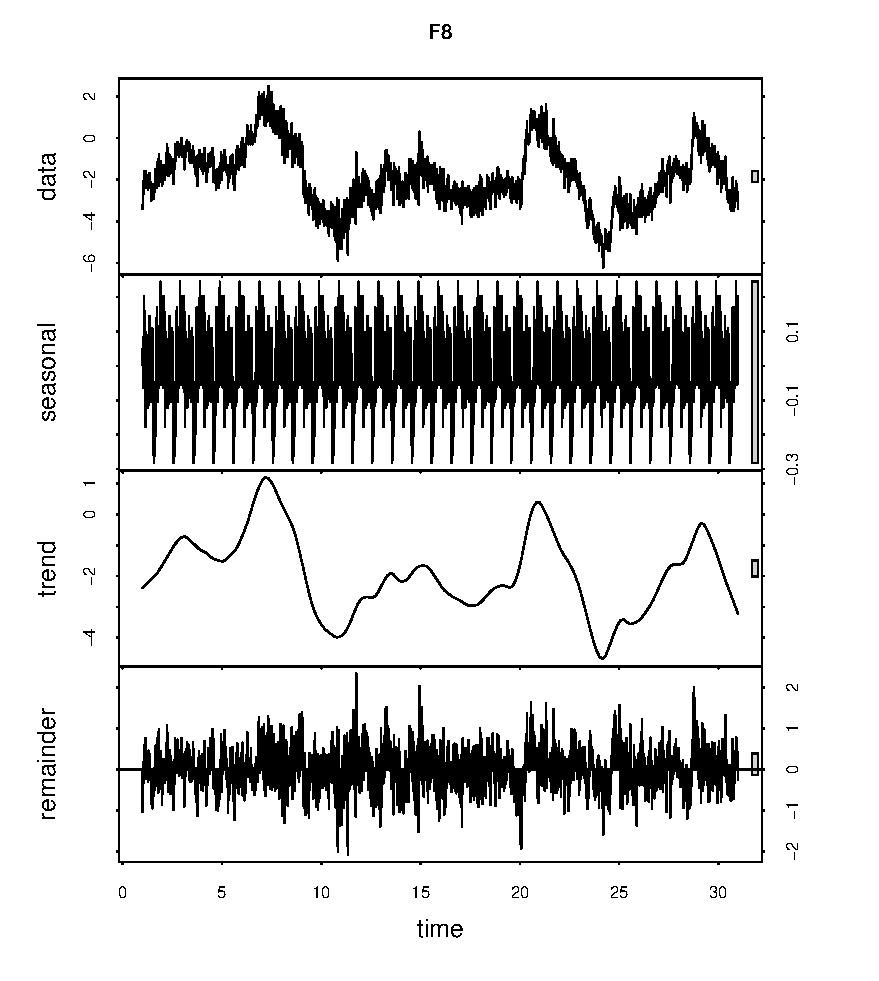
\includegraphics[width=0.5\linewidth]{./trabajo2/stl_n_f8.pdf} 
%\end{figure}
%\end{frame}
%
%%estacionalidad: frecuencia de muestreo
%
%\begin{frame}\frametitle{Casos de estudio: posible deterioro}
%\begin{figure}[h]
%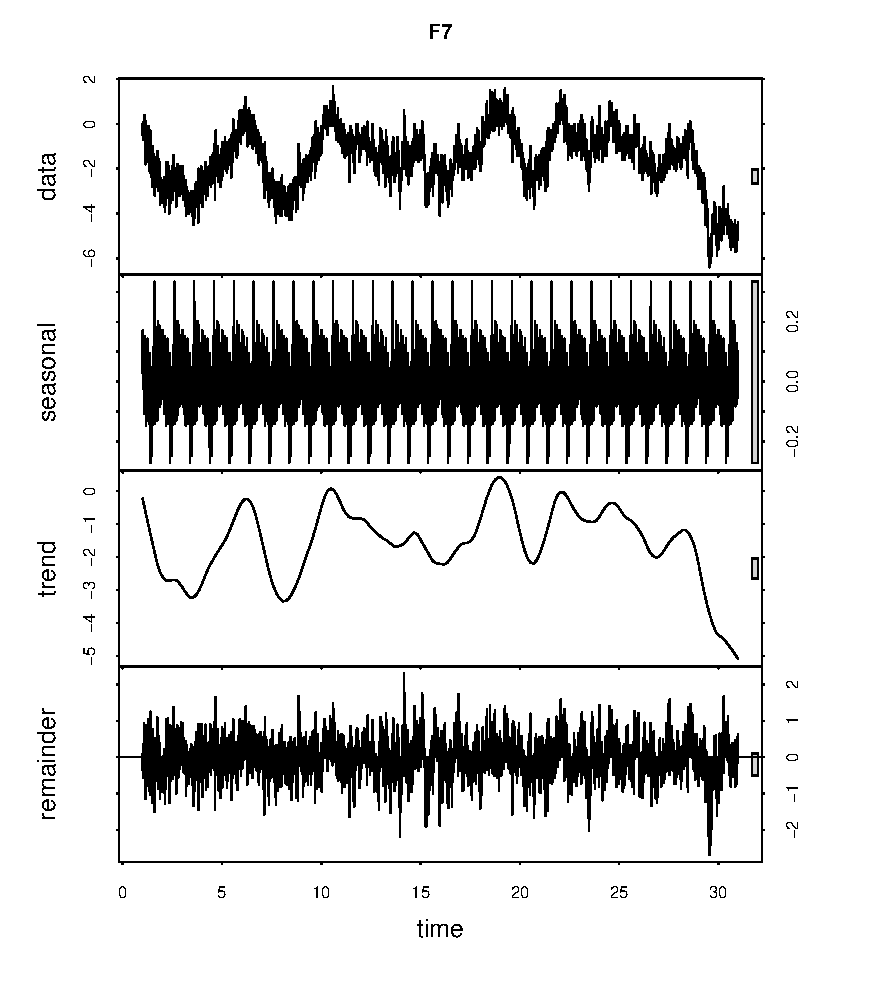
\includegraphics[width=0.5\linewidth]{./trabajo2/stl_d_f7.pdf} 
%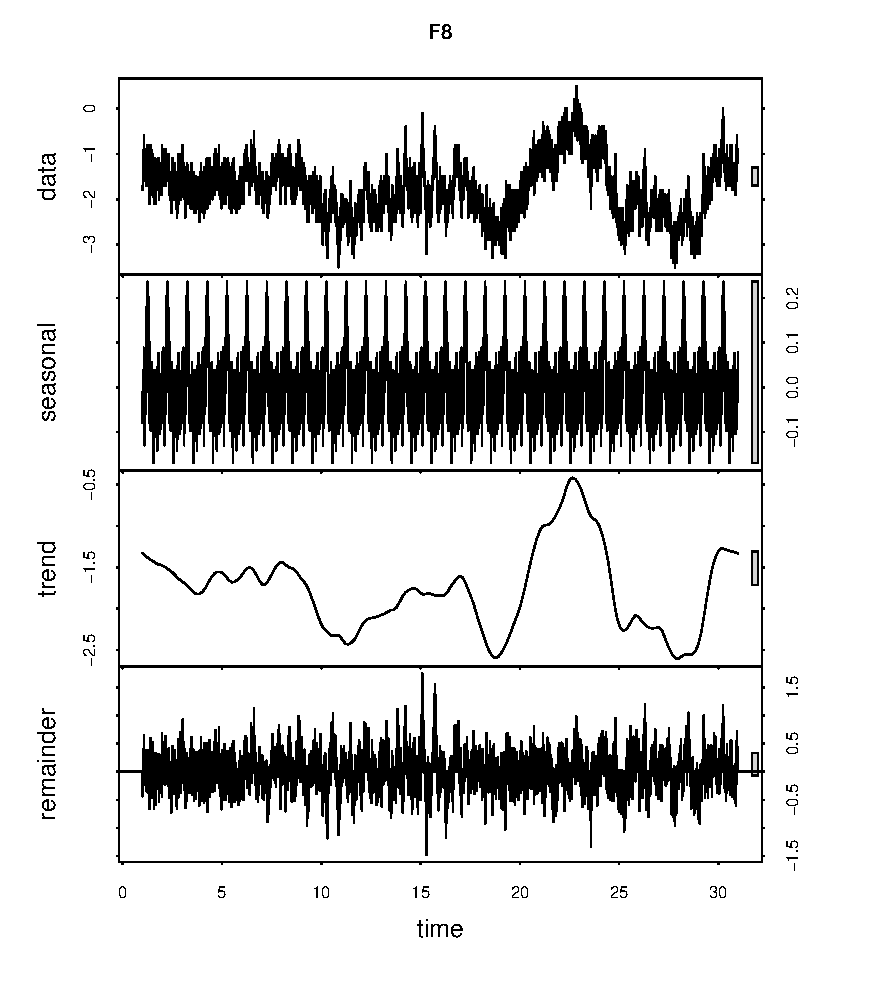
\includegraphics[width=0.5\linewidth]{./trabajo2/stl_d_f8.pdf} 
%\end{figure}
%\end{frame}
%
%%%%%%%%%%%%%%%%%%%%%%%%%%%%%%%%%%%%%%%%%%%
%%%%%%%%%%%%%%%%%%%%%%%%%%%%%%%%%%%%%%%%%%%
%
%\section{Priestley-Subba Rao}
%
%\begin{frame}\frametitle{Proceso arm\'onico de Priestley}
%Al trabajar con se\~nales el\'ectricas, parece natural una representaci\'on del tipo
%
%\begin{equation*}
%X_t = \sum_{i=1}^{K} A_i \cos \left( \omega_i t + \phi_i \right)
%\end{equation*}
%
%Donde
%\begin{description}
%\item[$K$] $\in \mathbb{N}$
%\item[$A_i$] $\in \mathbb{R}$, {amplitudes}
%\item[$\omega_i$] $\in \mathbb{R}$, {frecuencias}
%\item[$ \phi_i $] va iid con distribuci\'on uniforme en $[-\pi,\pi]$
%\end{description}
%\end{frame}
%
%%%%%%%%%%%%%%%%%%%%%%%%%%%%%%%%%%%%%%%%%%%
%%%%%%%%%%%%%%%%%%%%%%%%%%%%%%%%%%%%%%%%%%%
%
%\begin{frame}\frametitle{Proceso arm\'onico de Priestley (ver. continua)}
%%Considerado \textit{todas} las frecuencias en $[-\pi,\pi]$
%Al trabajar con se\~nales el\'ectricas, parece natural una representaci\'on del tipo
%
%\begin{equation*}
%X_t = \int_{-\pi}^{\pi} A(\omega) e^{i\omega t} \, d\xi(\omega)
%\end{equation*}
%
%Donde
%\begin{description}
%\item[$\omega$] Frecuencia puntual
%\item[$\xi(\omega)$] \textit{va. infinitesimal}, asociada con $\omega$
%\item[$A(\omega)$] Amplitud en $\omega$
%\end{description}
%\end{frame}
%
%%%%%%%%%%%%%%%%%%%%%%%%%%%%%%%%%%%%%%%%%%%
%%%%%%%%%%%%%%%%%%%%%%%%%%%%%%%%%%%%%%%%%%%
%
%\begin{frame}\frametitle{Representaci\'on espectral}
%Se tiene un proceso $X_t$, con $E[X_t]<\infty$, $E[T_t^{2}]<\infty$,
%%y que consid\'erese la representaci\'on 
%%Sup\'ongase que es posible expresar
%
%\begin{equation*}
%X_t = \int_{-\pi}^{\pi} A_t(\omega) e^{i\omega t} \, d\xi(\omega)
%\end{equation*}
%
%\begin{description}
%\item[$\{ \xi(\omega) \}$] Familia de procesos ortogonales con {{ $E \lvert d \xi(\omega) \lvert^{2} = \mu(\omega)$ }}
%\item[$A_t(\omega)$] Su tr. de Fourier en $t$ tiene un m\'aximo absoluto en 0
%\end{description}
%
%\pause
%Se define el \textbf{espectro evolutivo} de $X_t$, con respecto a la la familia, como
%\begin{equation*}
%f_t(\omega) = \lvert A_t(\omega) \lvert^{2}
%\end{equation*}
%\end{frame}
%
%%%%%%%%%%%%%%%%%%%%%%%%%%%%%%%%%%%%%%%%%%%
%%%%%%%%%%%%%%%%%%%%%%%%%%%%%%%%%%%%%%%%%%%
%
%\begin{frame}\frametitle{Test de Priestley-Subba Rao}
%Sup\'ongase que puede expresarse
%\begin{equation*}
%X_t = \int_{-\pi}^{\pi} A_t(\omega) e^{i\omega t} \, d\xi(\omega)
%\end{equation*}
%
%\pause
%\begin{center}
%$X_t$ es estacionaria $\Rightarrow A_t(\omega)$ es constante $\Rightarrow f_t(\omega)$ es constante
%\end{center}
%
%\pause
%La contrapositiva
%\begin{center}
%$f_t(\omega)$ no constante $\Rightarrow X_t$ \textbf{no} es estacionaria
%\end{center}
%
%\underline{Por hacer:} Encontrar un \textit{buen} estimador para $f_t$
%\end{frame}
%
%%%%%%%%%%%%%%%%%%%%%%%%%%%%%%%%%%%%%%%%%%%
%%%%%%%%%%%%%%%%%%%%%%%%%%%%%%%%%%%%%%%%%%%
%
%\begin{frame}[fragile]\frametitle{Estimador de doble ventana (sin detalles)}
%
%\begin{center}
%\begin{tabular}{cc}
%\includemovie{5em}{5em}{./trabajo2/priestley_spectra_full.gif}
%\includemovie{5em}{5em}{./trabajo2/priestley_spectra_small.gif}
%\end{tabular} 
%\end{center}
%
%%Por hacer: reescribir las ecuaciones del paper priestley68
%\end{frame}
%
%%%%%%%%%%%%%%%%%%%%%%%%%%%%%%%%%%%%%%%%%%%
%%%%%%%%%%%%%%%%%%%%%%%%%%%%%%%%%%%%%%%%%%%
%
%\begin{frame}
%\begin{figure}[h]
%%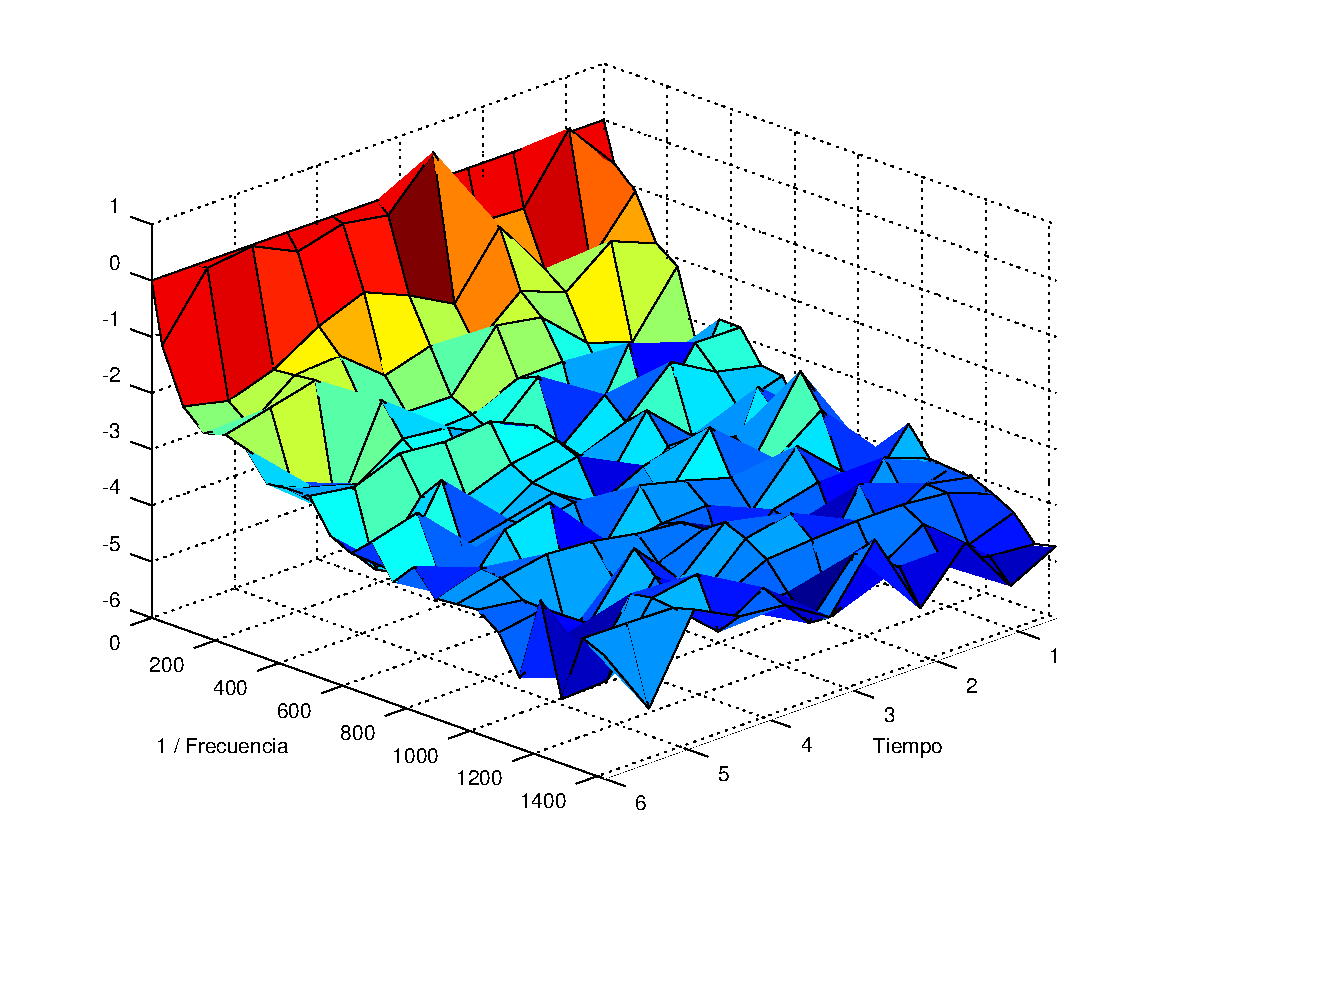
\includegraphics[width=\linewidth]{./trabajo2/ejemplo_espectro.pdf} 
%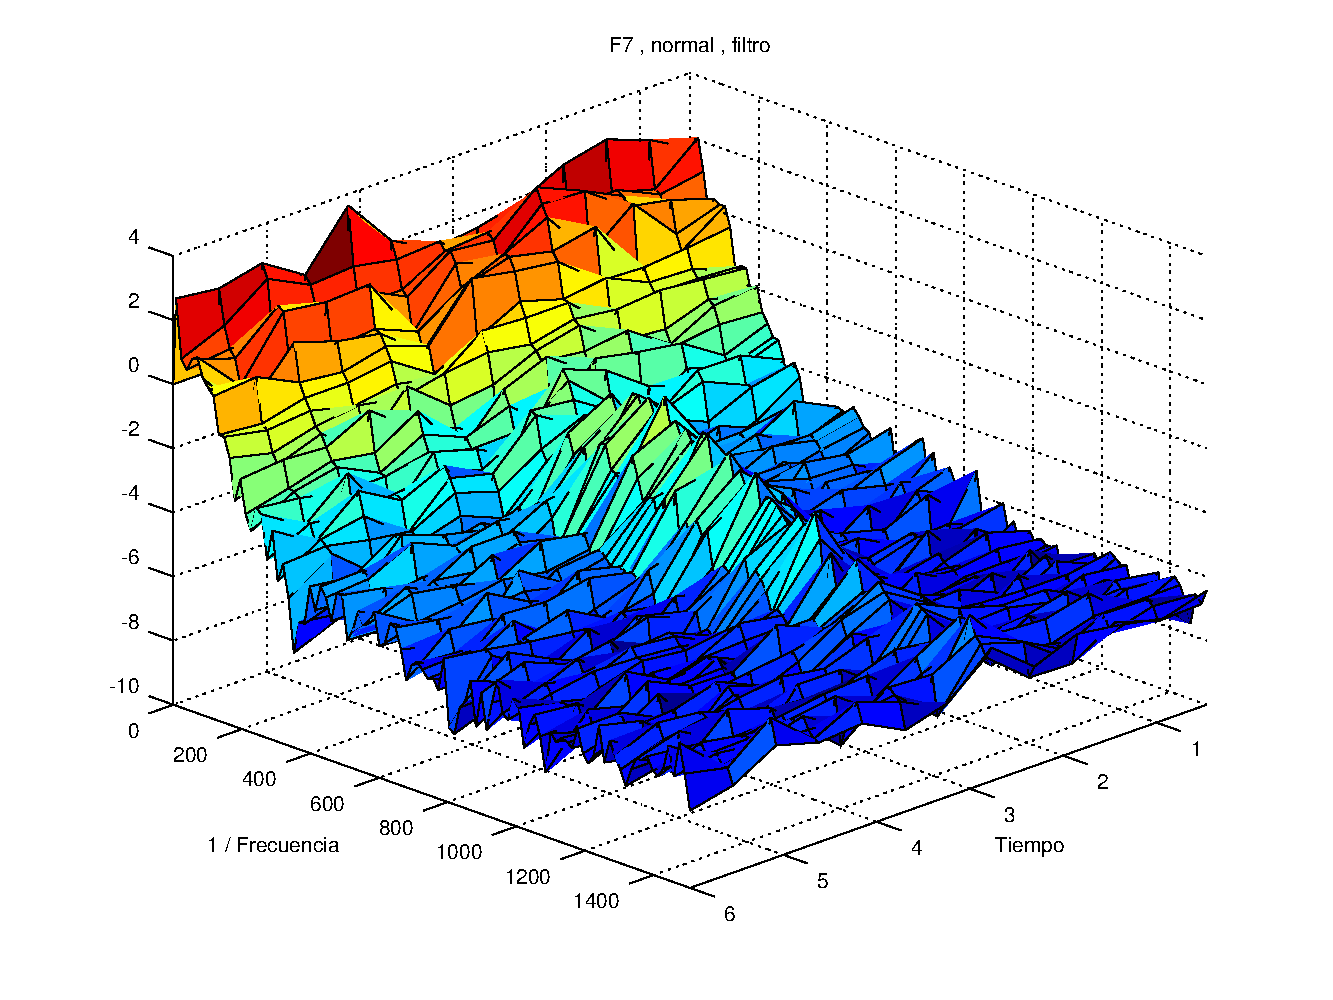
\includegraphics[width=\linewidth]{./trabajo2/n7f.pdf}
%\end{figure}
%\end{frame}
%
%%%%%%%%%%%%%%%%%%%%%%%%%%%%%%%%%%%%%%%%%%%
%%%%%%%%%%%%%%%%%%%%%%%%%%%%%%%%%%%%%%%%%%%
%
%\begin{frame}%\frametitle{Estad\'istico $Y$}
%Se define $Y_{i,j} = \log \left( \widehat{f_{t_i}}(\omega_j) \right)$, con las siguientes propiedades
%
%\begin{equation*}
%E\left[ Y_{i,j} \right] \thicksim \log \left( f_{t_i}(\omega_j) \right)
%\hspace{4em}
%\text{Var}\left( {Y\left(t,\omega\right)}\right) \thicksim \sigma^{2}
%\end{equation*}
%
%Luego, puede escribirse $Y_{i,j} = \log \left( f_{t_i}(\omega_j) \right) + \varepsilon_{i,j}$,
%con $\varepsilon_{i,j}$ va iid
%\vspace{2em}
%
%\pause
%Usando un test ANOVA --de varianza conocida-- se puede saber si $\varepsilon$
%\vspace{-1em}
%\begin{itemize}
%\item Tiene marginales
%\item Constante sobre el tiempo
%\item Constante sobre las frecuencias
%\end{itemize}
%\end{frame}
%
%%%%%%%%%%%%%%%%%%%%%%%%%%%%%%%%%%%%%%%%%%%
%%%%%%%%%%%%%%%%%%%%%%%%%%%%%%%%%%%%%%%%%%%
%
%\begin{frame}[fragile]
%\begin{lstlisting}
%Priestley-Subba Rao stationarity Test for datos
%-----------------------------------------------
%Samples used              : 3072 
%Samples available         : 3069 
%Sampling interval         : 1 
%SDF estimator             : Multitaper 
%  Number of (sine) tapers : 5 
%  Centered                : TRUE 
%  Recentered              : FALSE 
%Number of blocks          : 11 
%Block size                : 279 
%Number of blocks          : 11 
%p-value for T             : 0.4130131 
%p-value for I+R           : 0.1787949 
%p-value for T+I+R         : 0.1801353 
%\end{lstlisting}
%\end{frame}
%
%%%%%%%%%%%%%%%%%%%%%%%%%%%%%%%%%%%%%%%%%%%
%%%%%%%%%%%%%%%%%%%%%%%%%%%%%%%%%%%%%%%%%%%
%
%\begin{frame}[fragile]
%\begin{tabular}{cc}
%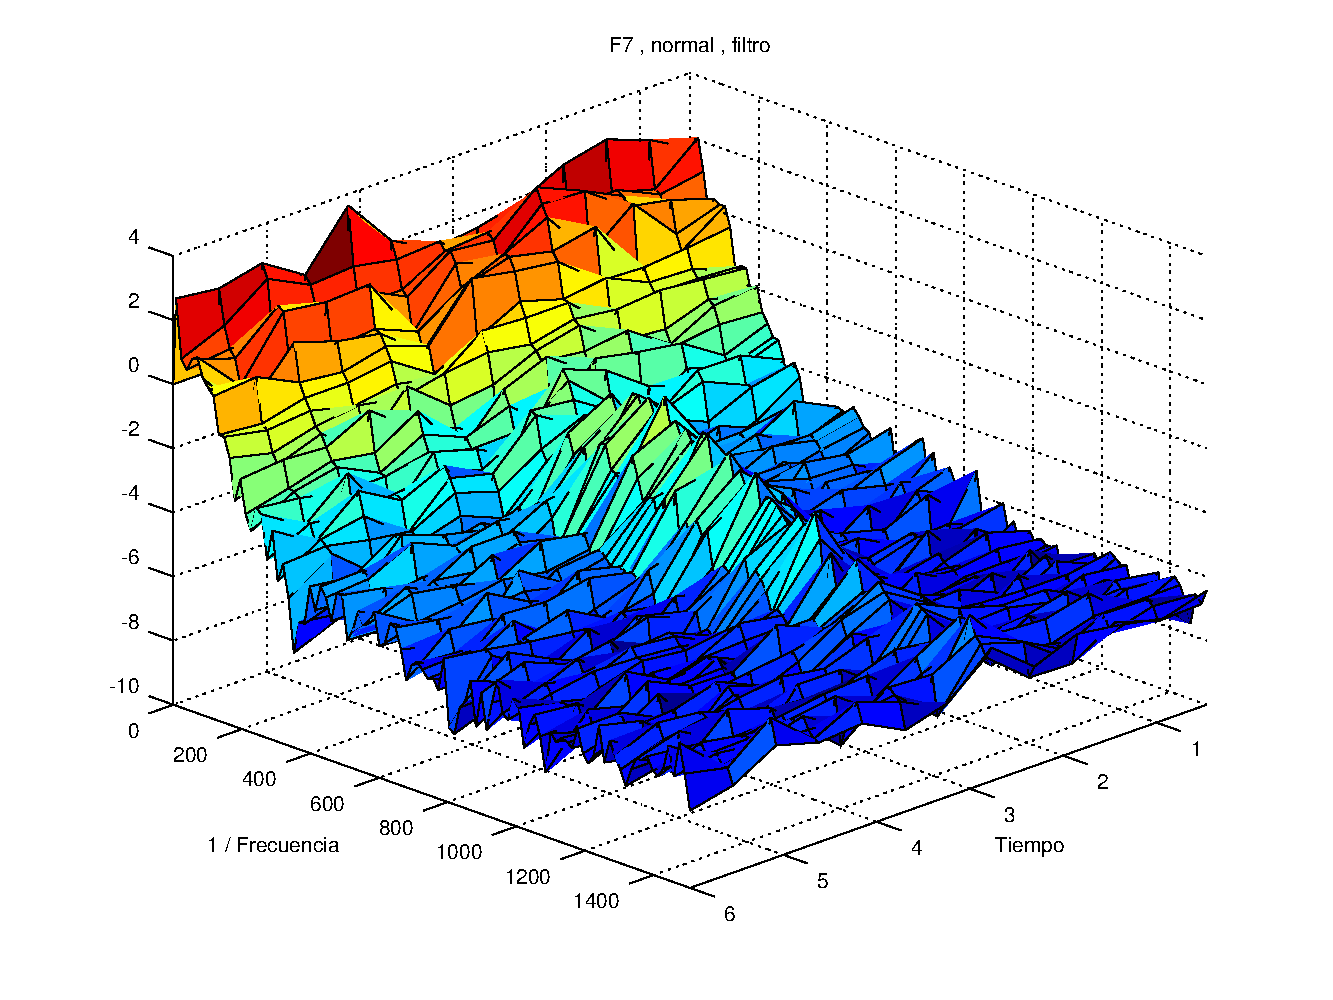
\includegraphics[width=0.5\linewidth]{./trabajo2/n7f.pdf} 
%&
%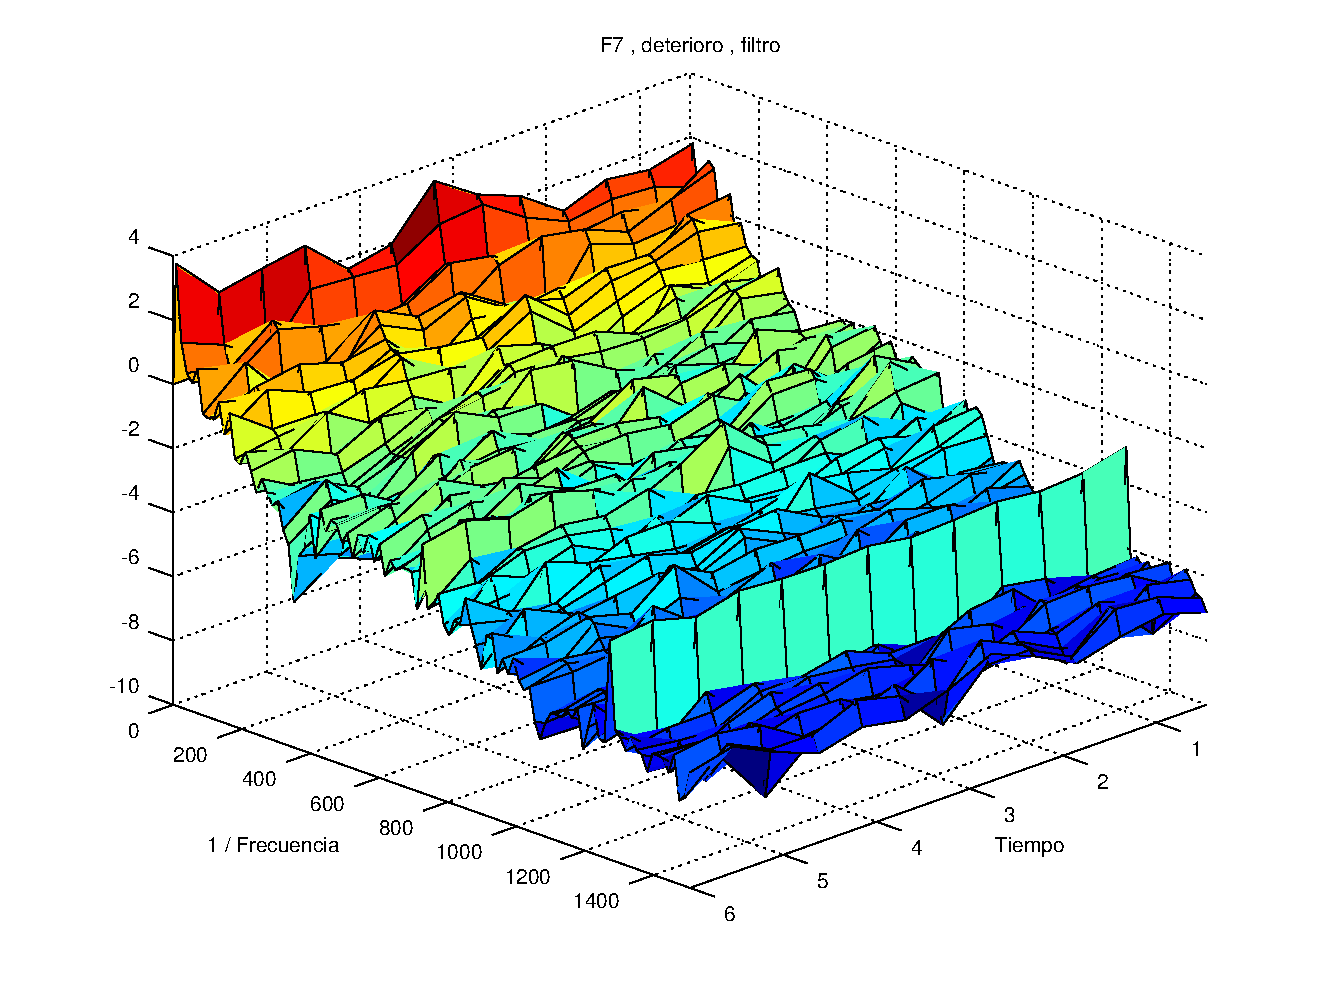
\includegraphics[width=0.5\linewidth]{./trabajo2/d7f.pdf} 
%\\
%\begin{lstlisting}
%T      : 0 
%I+R    : 0 
%T+I+R  : 0 
%\end{lstlisting}
%&
%\begin{lstlisting}
%T      : 4.36434e-07 
%I+R    : 0.0001575723 
%T+I+R  : 6.98897e-06 
%\end{lstlisting}
%\end{tabular}
%\end{frame}
%
%%%%%%%%%%%%%%%%%%%%%%%%%%%%%%%%%%%%%%%%%%%
%%%%%%%%%%%%%%%%%%%%%%%%%%%%%%%%%%%%%%%%%%%
%
%\begin{frame}[fragile]
%\begin{tabular}{cc}
%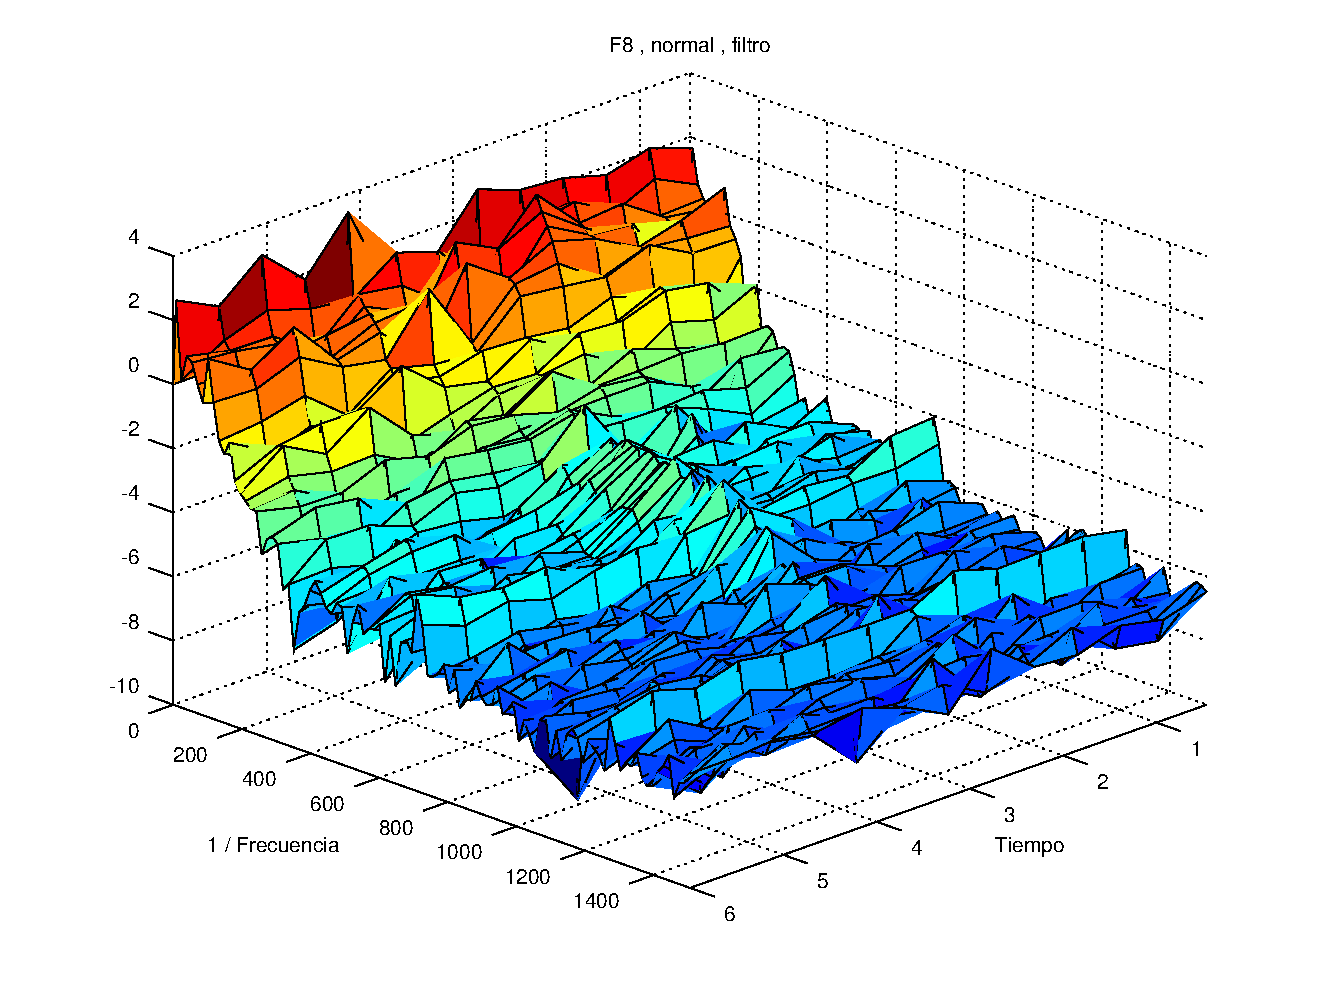
\includegraphics[width=0.5\linewidth]{./trabajo2/n8f.pdf} 
%&
%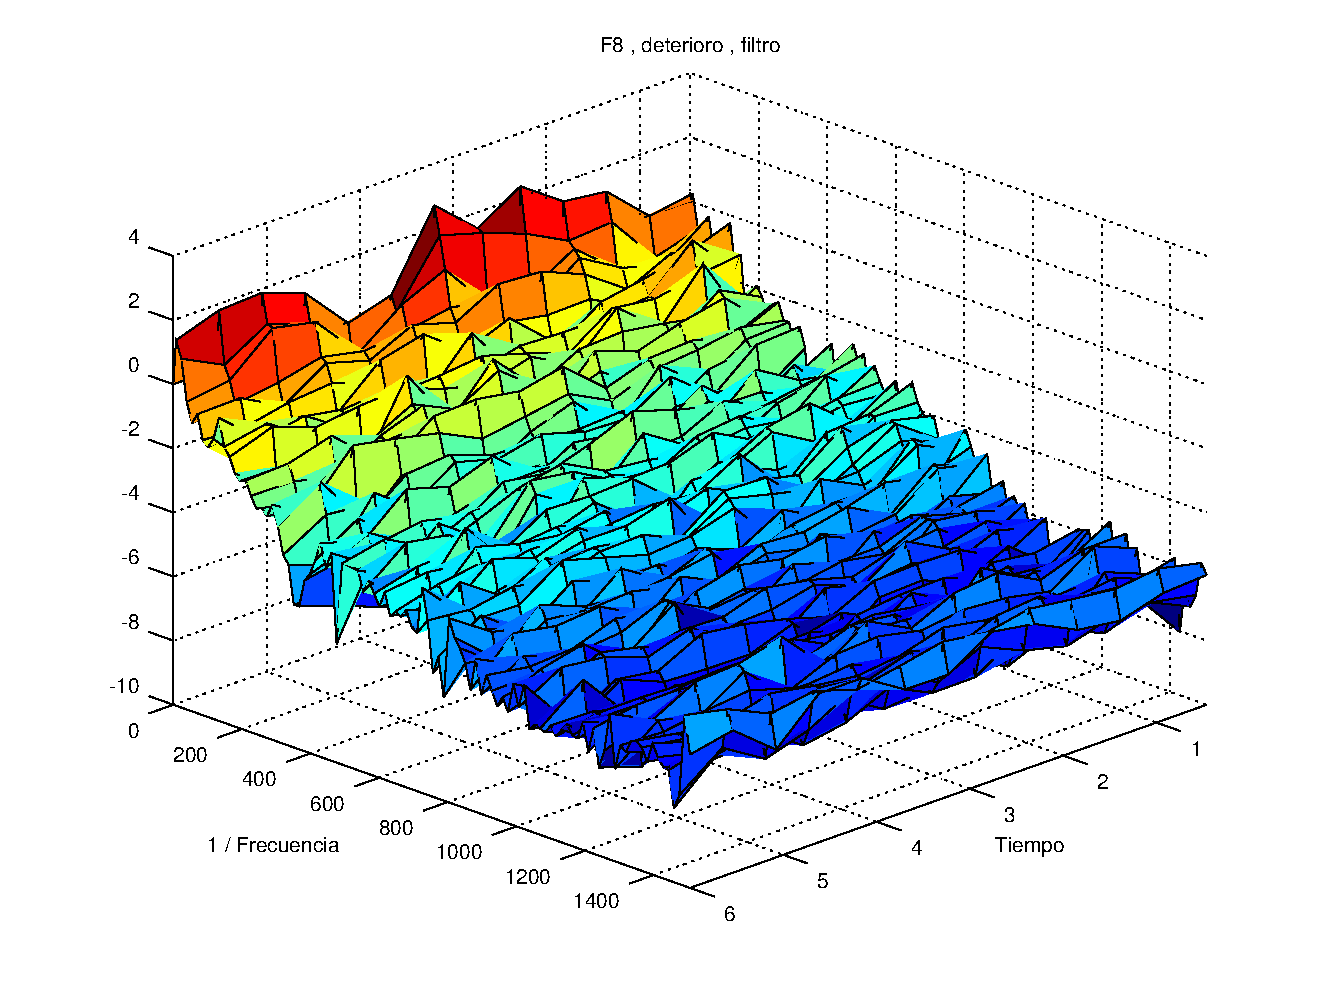
\includegraphics[width=0.5\linewidth]{./trabajo2/d8f.pdf} 
%\\
%\begin{lstlisting}
%T      : 0 
%I+R    : 5.787895e-09 
%T+I+R  : 0 
%\end{lstlisting}
%&
%\begin{lstlisting}
%T      : 0.00332259 
%I+R    : 0.03502537 
%T+I+R  : 0.01598073 
%\end{lstlisting}
%\end{tabular}
%\end{frame}
%
%%%%%%%%%%%%%%%%%%%%%%%%%%%%%%%%%%%%%%%%%%%
%%%%%%%%%%%%%%%%%%%%%%%%%%%%%%%%%%%%%%%%%%%
%
%\begin{frame}\frametitle{Conclusi\'on}
%El an\'alisis de la estacionariedad d\'ebil en registros de sue\~no MOR
%muestra diferencias para el grupo con Deterioro Cognitivo (DC)
%en comparaci\'on con el grupo control, lo que indica que el an\'alisis de estacionariedad es
%eficiente como marcator para detectar el DC durante el sue\~no MOR en adultos mayores.
%\end{frame}
%
%%%%%%%%%%%%%%%%%%%%%%%%%%%%%%%%%%%%%%%%%%%
%%%%%%%%%%%%%%%%%%%%%%%%%%%%%%%%%%%%%%%%%%%
%
%\begin{frame}\frametitle{Agradecimientos}
%\begin{figure}
%\includegraphics[width=0.6\linewidth]{cerebro.jpg}
%\end{figure}
%\begin{itemize}
%\item A la Dra. Erika Rodr\'guez Torres, por el \textbf{gran} apoyo prestado
%\item A la Dra. G\'enesis Roc\'io V\'azquez-Tagle Gallegos, por las bases de datos
%\end{itemize}
%%[Tambi\'en deber\'ia mencionarse los datos obtenidos]
%\end{frame}

%%%%%%%%%%%%%%%%%%%%%%%%%%%%%%%%%%%%%%%%%%
%%%%%%%%%%%%%%%%%%%%%%%%%%%%%%%%%%%%%%%%%%

%\begin{frame}[allowframebreaks]
%\frametitle{Bibliograf\'ia}
%%\nocite{*}
%\footnotesize{
%%\bibliography{referencias}
%\bibliography{referencias_estacionariedad,referencias_fisiologia,referencias_otros,referencias_mixto}{}
%\bibliographystyle{apalike-es}
%%\bibliographystyle{abbrv}
%}
%\end{frame}

\end{document}